\documentclass[../PHYS306Notes.tex]{subfiles}

\begin{document}
\section{Lecture 33}
\subsection{Lecture Notes - Lyapunov Exponents, Bifurcation Diagrams, State-Space orbits, and Poincare Sections}
\subsubsection{Period doubling cascade - "Route to Chaos"}
Period doubles each time the driving strength of the driven damped pendulum is increased past $\gamma_n$:
\[\delta = \lim_{n\rightarrow\infty}\frac{\gamma_{n-1} - \gamma_{n-2}}{\gamma_n - \gamma_{n-1}} = 4.6692016\ldots\]
This is the universal "Feigenbaum number".
\subsubsection{The driven damped pendulum revisisted}
We return to the driven damped pendlum from last day. Giving two pendulums driving strengths of $\gamma = 1.503$, and one with initial phase of $\phi_0 = 0$ and the other with $\phi_0 = 0.005$, we can see that after time, the trajectories begin to diverge significantly.
\begin{center}
    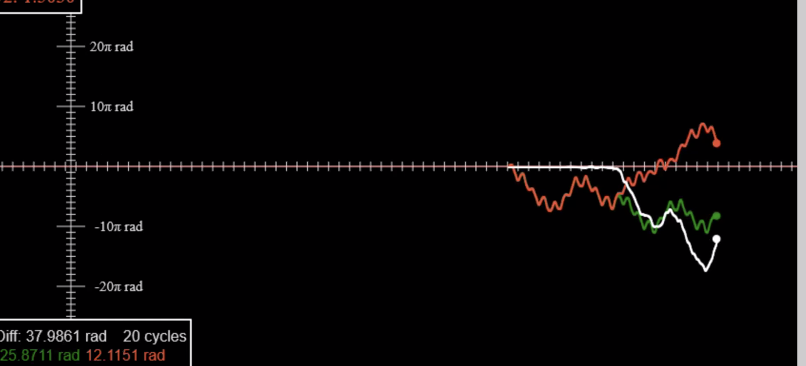
\includegraphics[scale=0.7]{Lecture-33/l33-img1.png}
\end{center}
With a driving strength of 1.077, and an initial phase shift of $-28$, we see that there is definitely a divergence in the two trajectories, but it looks periodic. 
\begin{center}
    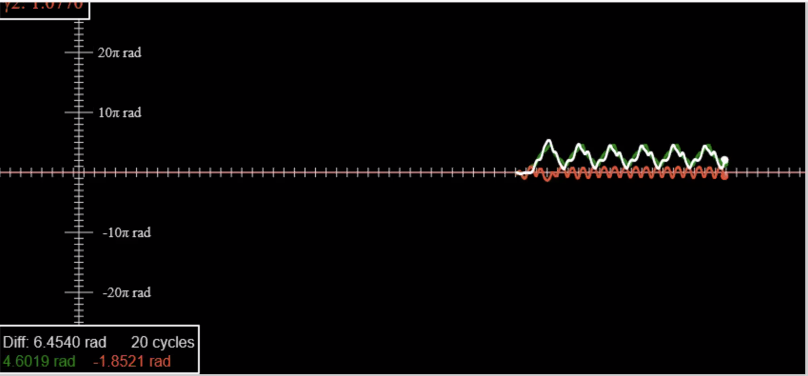
\includegraphics[scale=0.7]{Lecture-33/l33-img2.png}
\end{center}
With $\Delta \phi = -27$, the difference is different from $\Delta \phi = -28$ but still periodic. With $\Delta \phi = -29$, we see that we actually reach a constant difference:
\begin{center}
    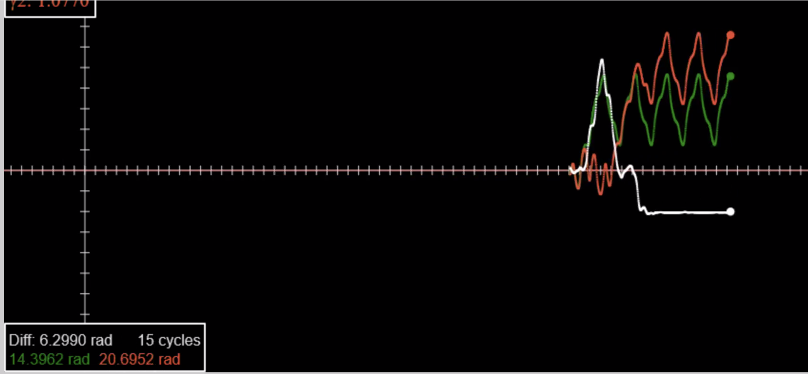
\includegraphics[scale=0.7]{Lecture-33/l33-img3.png}
\end{center}
With a slightly different driving strength, we see:
\begin{center}
    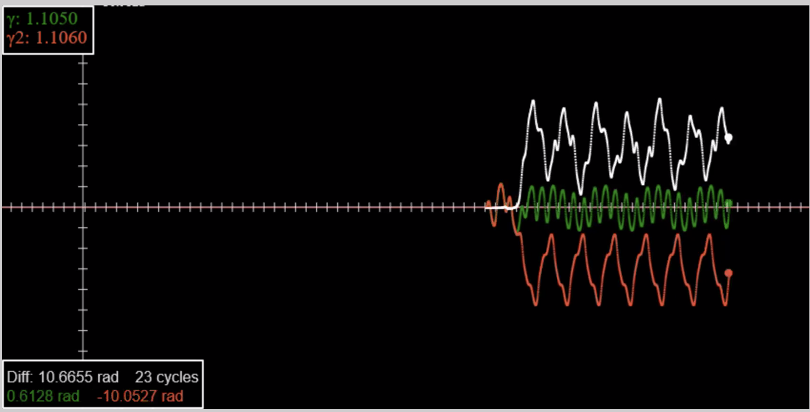
\includegraphics[scale=0.7]{Lecture-33/l33-img4.png}
\end{center}
We recognize that we are slightly further into the chaotic regime; looking at the difference between the two pendulums, we see that there is no repeated pattern (there are slight differneces between cycles, so there doesn't appear to be periodic/perfect repetition).

\subsubsection{Sensitivity to Initial Conditions \& Lyapunov Exponents}
$\Phi(t) = \Phi_2(t) - \Phi_1(t)$ os the difference between two solutions with slightly different initial conditions. For linear oscillations,
\[\Delta \Phi(t) = D\exp(-\beta t)\cos(\omega t - \delta)\]
In general:
\[\Delta \Phi(t) \sim K\exp(\lambda t)\]
$\lambda$ is the Lyapunov exponent, with periodic motion when it is negative and chaotic motion when it is positive. It is often best to plot $\log\abs{\Delta \Phi(t)} \sim \lambda t + \text{Const.}$ to see what happens with time.Doing so, we should either see a line with a positive or negative slope, depending on whether the trajectory is divergent (chaotic) or convergent (periodic) respectively. Plotting this for our two driven damped pendulums, we see:
\begin{center}
    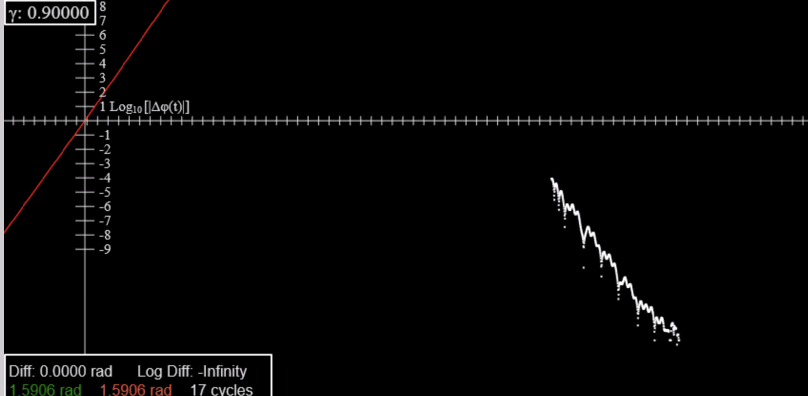
\includegraphics[scale=0.7]{Lecture-33/l33-img5.png}
\end{center}
The peaks follow the linear trend, and the dips correspond to when $\Delta \Phi$ becomes negative. For driving of 1.07 (higher), we se that we still have convergence, but the Lyapunov exponent is less negative; it takes longer for the difference between the two osicllators to vanish.
\begin{center}
    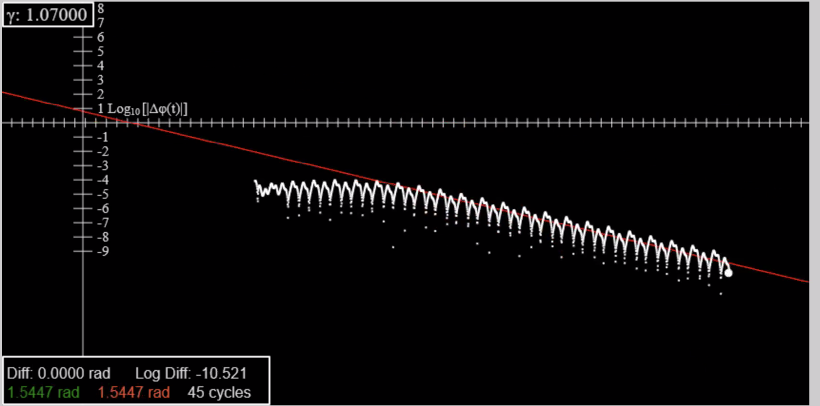
\includegraphics[scale=0.7]{Lecture-33/l33-img6.png}
\end{center}

Ramping it up to a driving strength of 1.105, we get into the Chaotic regime, where the overall slope is positive:
\begin{center}
    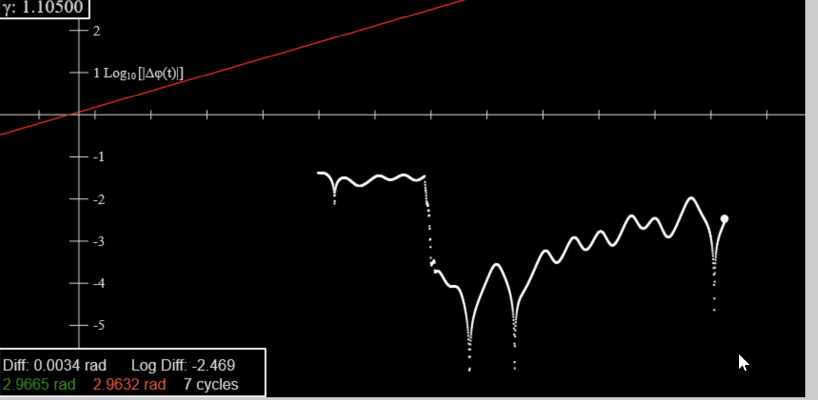
\includegraphics[scale=0.7]{Lecture-33/l33-img7.png}    
\end{center}
But bringing it up to 1.13, we actually go back to the non-chaotic regime:
\begin{center}
    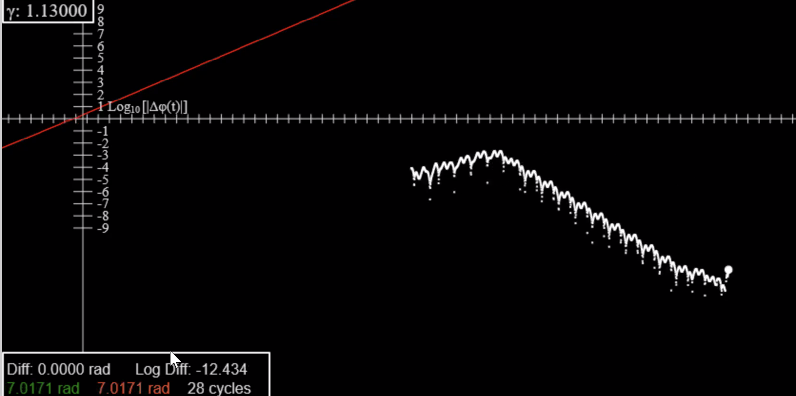
\includegraphics[scale=0.7]{Lecture-33/l33-img8.png}    
\end{center}

\subsubsection{Bifurcation Diagrams}
It gets quite confusing as to when the motion is chaotic, or not! A nice way of visualizing this is with a bifurcation diagram. We plot the driving strength on the $x$ axis and $\phi(t)$ on the y axis:
\begin{center}
    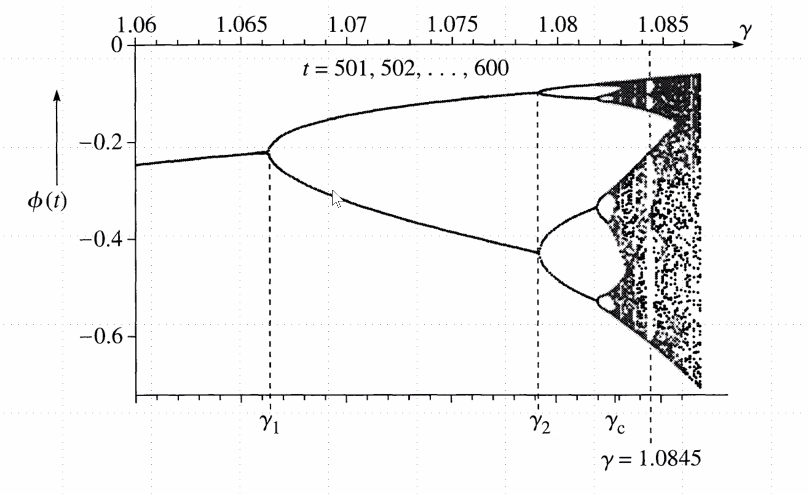
\includegraphics[scale=0.6]{Lecture-33/l33-img9.png}
\end{center}
Here, we only plot the phase at specific times. If the motion is periodic and we take pictures at specific intervals, we always end up at the same point (e.g. before $\gamma_1$). However, past $\gamma_1$, we get period doubling and hence taking snapshots of the pendulum at the original period, we will now see two periods. Past $\gamma_2$, we see 4 different values, and so on. Past $\gamma = 1.0845$ we get into the chaotic regime. There is one more subtlety; once we increase the driving strength past a certain point, the pendulum can roll over the top, so the angle can go to infinity; this is a bit inconvenient! Although we could make the phase $2\pi$ periodic, another fix is to just plot the velocity as  a function of the driving strength:
\begin{center}
    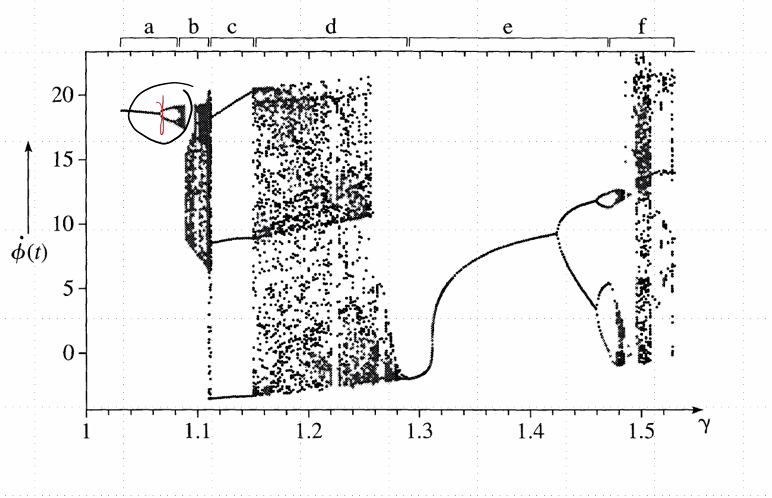
\includegraphics[scale=0.6]{Lecture-33/l33-img10.png}
\end{center}
We can see distint regions of periodicity and chaos; the circled part of $a$ was the period doubling we were studying earlier, $b$ is chaotic, then $c$ goes back to regular/periodic motion, then it gets chaotic for a while $d$, then we have regular motion for a while $e$ and so on. These diagrams can be quite useful to see these regions of chaos and regularity.

\subsubsection{State Space Orbits}
Very similar to phase space diagrams we did with Hamiltonian mechanics, but now we plot $\dot{\phi}$ versus $\phi$. Looking at this plot letting it run for a little while, we can see that there are four different cycles. (4 different trajectories); we are in a period 4 scenario. 
\begin{center}
    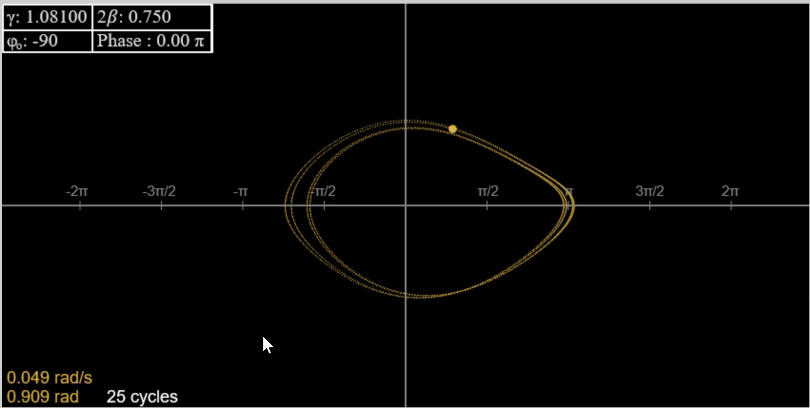
\includegraphics[scale=0.7]{Lecture-33/l33-img11.png}
\end{center}
Going to 1.0826, we see that after the initial transience, looking very carefully we have a period 8 scenario:
\begin{center}
    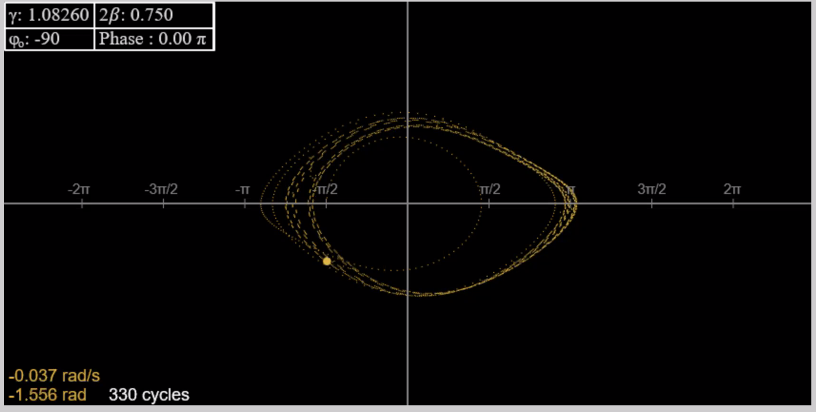
\includegraphics[scale=0.7]{Lecture-33/l33-img12.png}
\end{center}
And for 1.087 we get period 16 and so on.
\begin{center}
    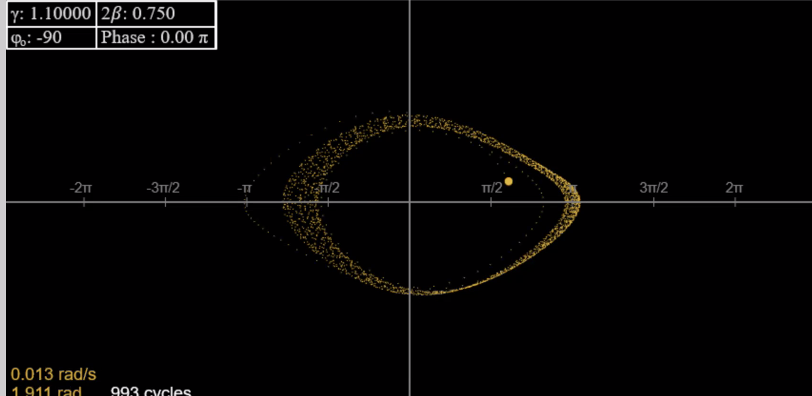
\includegraphics[scale=0.7]{Lecture-33/l33-img13.png}
\end{center}
As we increase the driving strength even further, the motion becomes truly aperiodic.But, increasing it back to 1.1, we get back to a periodic region (where the pendulum starts to roll over):
\begin{center}
    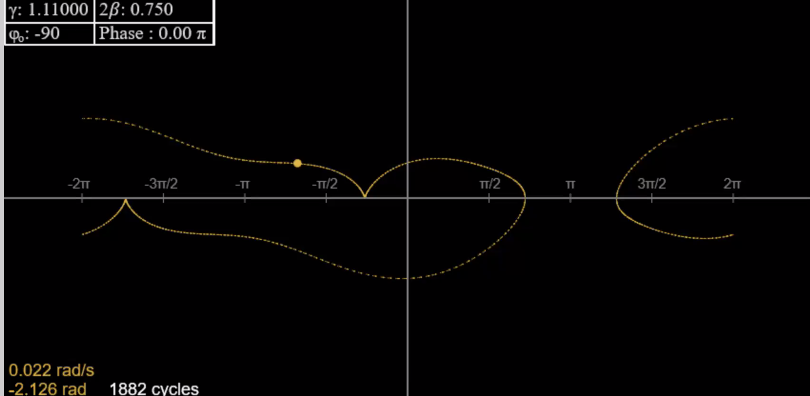
\includegraphics[scale=0.7]{Lecture-33/l33-img14.png}
\end{center}
And increasing it further, the motion gets chaotic again:
\begin{center}
    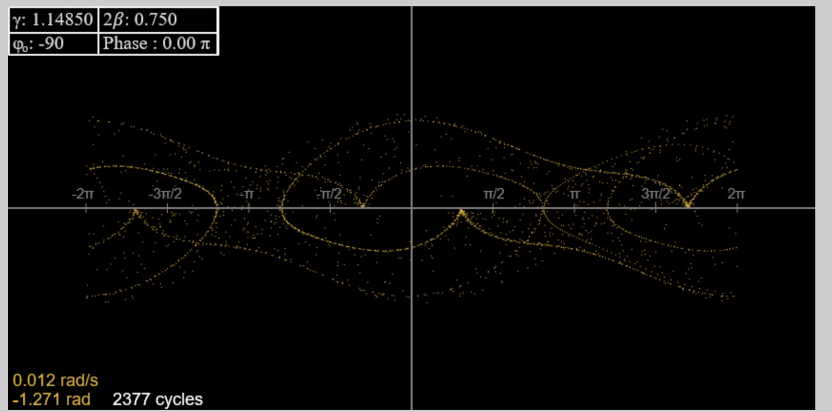
\includegraphics[scale=0.7]{Lecture-33/l33-img15.png}
\end{center}
\subsubsection{Poincare Sections}
We can plot a point per cycle to get a Poincare section:
\begin{center}
    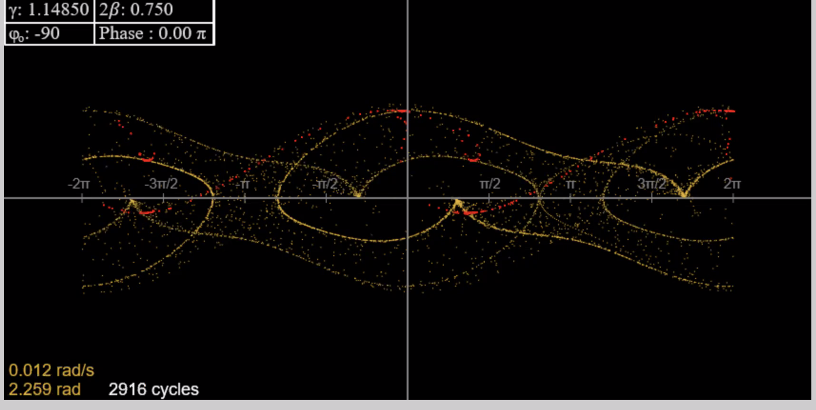
\includegraphics[scale=0.7]{Lecture-33/l33-img16.png}
    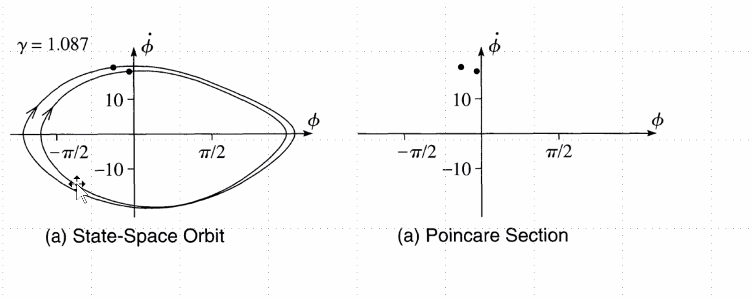
\includegraphics[scale=0.7]{Lecture-33/l33-img17.png}
\end{center}
So for the 4-period case, we expect to see 4 dots, which is indeed the case (though two are close together in the below plot):
\begin{center}
    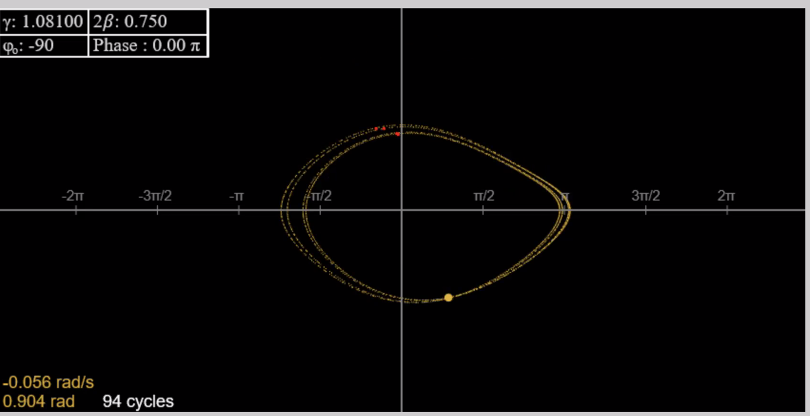
\includegraphics[scale=0.7]{Lecture-33/l33-img18.png}
\end{center}
Pictured below is a strange attractor:
\begin{center}
    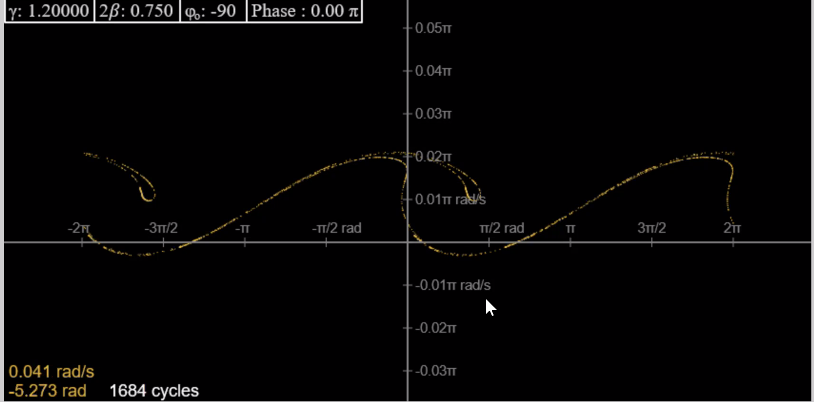
\includegraphics[scale=0.7]{Lecture-33/l33-img19.png}
\end{center}
This is actually a fractal; fractals have scale invariance/self-similarity.

\subsubsection{The Logistic map}
The logistic map is defined as $x_{t+1} \mapsto rx_t(1 - x_t)$, describing the reproduction and starvation of a population. Looking a the bifurcation diagram as we vary $r$, we see a similar development of chaotic behavior as the pendulum, due to the nonlinearity:
\begin{center}
    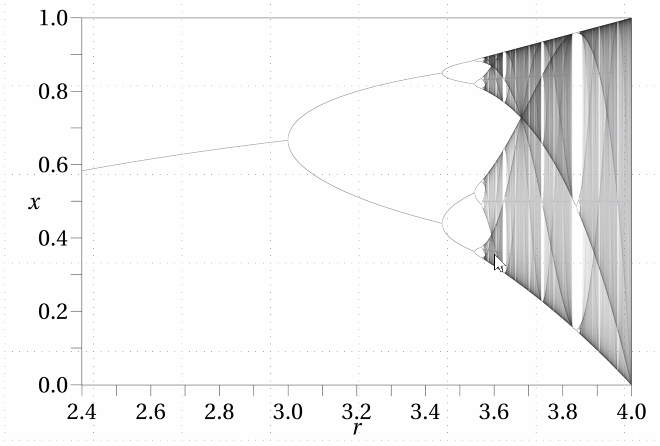
\includegraphics[scale=0.7]{Lecture-33/l33-img20.png}
\end{center}

\end{document}